\section{Archietttura del nuovo sistema}

Dopo aver raccolto e definito i requisiti per il nuovo sistema SRM attraverso varie riunioni con gli stakeholder e l'analisi del sistema attuale (SRP), è stato possibile progettare una nuova architettura per il sistema che permetta di soddisfare tali requisiti in modo efficiente e scalabile.


La nuova architettura proposta per il sistema SRM, riportata in figura \ref{fig:new-system-architecture}, è basata su un'architettura a microservizi, che consente una maggiore modularità, scalabilità e facilità di manutenzione rispetto all'architettura monolitica del sistema SRP attuale.

\begin{figure}[ht]
    \centering
    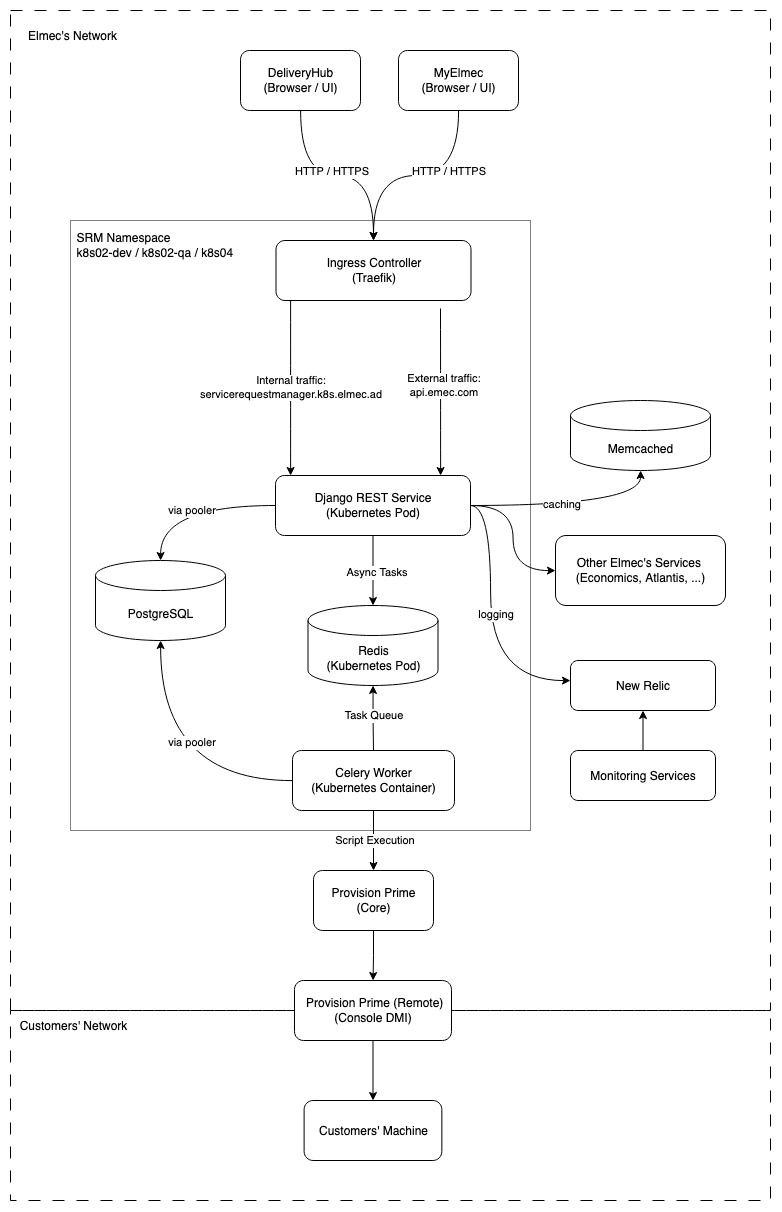
\includegraphics[width=1\textwidth]{images/architectural-redesign/System Design SRM.jpg}
    \caption{SRM System Architecture}
    \label{fig:new-system-architecture}
\end{figure}


\subsection{Componenti principali}
La nuova architettura del sistema SRM è composta dai seguenti componenti principali:
\begin{itemize}
    \item Frontend web (Vue.js)
    \item Servizi REST (Django REST Framework)
    \item Sistema di autenticazione e autorizzazione (PyElmecAuth)
    \item Database PostgreSQL
    \item Database Redis
    \item Sistema di caching (Memcached)
    \item Message Broker (Redis)
    \item Task Queue (Celery)
    \item Sistema di provisioning (Provision Prime)
    \item Sistema di monitoraggio e logging (New Relic)
    \item Sistemi di containerizzazione e orchestrazione dei container (Docker \& Kubernetes)
\end{itemize}

\subsubsection{Frontend}
Saranno sviluppati due frontend web separati per gli utenti finali e per gli amministratori di sistema, entrambi basati su Vue.js. Questi frontend comunicheranno con i servizi REST tramite API HTTP/HTTPS.

Grazie al fatto che la logica di business è stata spostata nei servizi REST, i frontend saranno più leggeri e facili da mantenere, permettendo una maggiore flessibilità nell'implementazione di nuove funzionalità e miglioramenti dell'interfaccia utente. Questo permette anche di integrare un'applicazione mobile in futuro, che potrà utilizzare le stesse API.

\subsubsection{Servizi REST}
REST (Representational State Transfer) è uno stile architetturale per la progettazione di servizi web che sfrutta i protocolli HTTP per la comunicazione tra client e server \cite{rest}. L'idea di base è che le risorse di un sistema (utenti, ordini, documenti, ecc.) vengano esposte attraverso un'interfaccia uniforme, tipicamente HTTP, usando \cite{rest}:
\begin{itemize}
    \item URL per identificare le risorse (\texttt{/api/catalog/actions/123/});
    \item Verbi HTTP per operare sulle risorse (\texttt{GET}, \texttt{POST}, \texttt{PUT}, \texttt{DELETE}, ...);
    \item Rappresentazioni delle risorse in formati standard (JSON, XML, ...).
\end{itemize}

I servizi REST saranno sviluppati utilizzando Django REST Framework, che offre un'architettura robusta e scalabile per la gestione delle API. 

Questi servizi saranno responsabili della logica di business, della gestione delle richieste degli utenti e dell'interazione con i database e altri componenti del sistema.

\subsubsection{Sistema di autenticazione e autorizzazione}
L'autenticazione e l'autorizzazione saranno gestite tramite la libreria PyElmecAuth sviluppata internamente, che si interfaccerà con il sistema di gestione delle identità aziendale per garantire un accesso sicuro e controllato ai servizi REST.

Sarà quindi necessario integrare in SRM un sistema di permessi granulare per garantire che gli utenti possano accedere solo alle risorse e alle funzionalità per cui sono autorizzati, basato sui ruoli definiti dall'Identity Provider aziendale.